\documentclass{article}

% if you need to pass options to natbib, use, e.g.:
%    \PassOptionsToPackage{numbers, compress}{natbib}
% before loading neurips_2019

% ready for submission
% \usepackage{neurips_2019}

% to compile a preprint version, e.g., for submission to arXiv, add add the
% [preprint] option:
 %  \usepackage[preprint]{neurips_2019}

% to compile a camera-ready version, add the [final] option, e.g.:
    \usepackage[final]{neurips_2019}

% to avoid loading the natbib package, add option nonatbib:
%    \usepackage[nonatbib]{neurips_2019}

\usepackage[utf8]{inputenc} % allow utf-8 input
\usepackage[T1]{fontenc}    % use 8-bit T1 fonts
\usepackage{hyperref}       % hyperlinks
\usepackage{url}            % simple URL typesetting
\usepackage{booktabs}       % professional-quality tables
\usepackage{amsfonts}       % blackboard math symbols
\usepackage{amsmath}
\usepackage{commath}
\usepackage{nicefrac}       % compact symbols for 1/2, etc.
\usepackage{microtype}      % microtypography
\usepackage{graphicx}
\graphicspath{ {./} }

\title{Statistical NLP - Project Proposal \\
Language Style Transfer with BERT}

% The \author macro works with any number of authors. There are two commands
% used to separate the names and addresses of multiple authors: \And and \AND.
%
% Using \And between authors leaves it to LaTeX to determine where to break the
% lines. Using \AND forces a line break at that point. So, if LaTeX puts 3 of 4
% authors names on the first line, and the last on the second line, try using
% \AND instead of \And before the third author name.

\author{%
  David Martuscello\\
  Courant Institute of Mathematical Sciences \\
  New York University\\
  \texttt{dm4350@nyu.edu} \\
  % examples of more authors
  \And
  Fang Han Cabrera\\
  Courant Institute of Mathematical Sciences \\
  New York University \\
  \texttt{fh643@nyu.ediu} \\
}
%%%%%%%%%%%%%%%%%%%%%%%%%%%%%%%%%%%%%%%%%%%%%%%%%
\begin{document}

\maketitle

\begin{abstract}
The task to transfer styles of texts is proved to be challenging because style and content interact in subtle ways and there's a lack of parallel data and reliable evaluation metrics. In response to the challenge, we embark on leveraging the state-of-art \textbf{BERT} model to improve the \textbf{encoder-decoder} model proposed in Zhou et al. (2018).
\end{abstract}

%%%%%%%%%%%%%%%%%%%%%%%%%%%%%%%%%%%%%%%%%%%%%%%%%
\section{Problem Setting}

Our project will be to reimplement and potentially expand upon the model discussed in the paper \emph{Language Style Transfer from Sentences with Arbitrary Unknown Styles} (Zhou et al. (2018)). The code from this paper is not publicly available, so our implementation will be strictly based on the research paper provided. Improvements or modifications may be included (see \ref{approach}). 
\paragraph{Language style transfer} is the task of generating a new sentence that preserves the content of the source sentence while emulating the style of a target domain. It is an important component of natural language generation that facilitates many NLP applications, such as automatic conversion of paper title to news title, which reduces the human effort in academic news report. For tasks like poetry
generation (Yan et al. 2013; Yan 2016; Ghazvininejad et al.2016), style transfer can be applied to generate poetry in different styles. 

\paragraph{Style and Content} A major challenge of style transfer is to separate
style from the content. In computer vision, Li et al. (2017) proposes an expression to distinguish style and content of a picture. However, this is under-explored in the NLP community. How to separate content from style in text remains an open research problem in text style transfer. One effective approach proposed in Shen et al. (2017) maps between sentences and continuous latent representations and then decompose the latent representations into style and content. The generative assumption adopted is as shown below, which we'll use in our implement.

\label{representation}
\begin{itemize}
\item \texttt{latent style variable} $y \sim p(y)$
\item \texttt{latent content variable} $z \sim p(z)$
\item \texttt{sentence} $x \sim p(x|y, z)$
\end{itemize}

\paragraph{Evaluation}is also a key challenge in style transfer. In machine translation and summarization, researchers use BLEU (Papineni et al. 2002) and ROUGE (Lin 2004) to compute the similarity between model outputs and the ground truth. However, we lack parallel data for style transfer to provide ground truth references for evaluation. The same problem also exists in style transfer in computer vision. To solve this problem, we adopt the evaluation metrics proposed by Fu et al.(2017), which will be discussed in detail in \ref{eval}.

%%%%%%%%%%%%%%%%%%%%%%%%%%%%%%%%%%%%%%%%%%%%%%%%%
\section{Related Work}
The task of style transfer has been predominantly explored by transferring style between images. However, many of the approaches used for image style transfer can be adapted to work with language. The model in Zhao et al. (2018) adapts the ideas of generative adversarial networks (GANs) as proposed in Goodfellow et al.(2014) and cycle consistency loss as proposed in Zhu et al. (2017).
Language style transfer has been performed before in Mueller er al. (2017)....
Most of the work in this area has made the assumption that the source domain has one consistent style and the target domain has its own consistent style. The paper we are focused on (Zhao et al. (2018)) loosens these assumptions to accept any source data, regardless of style. 


%%%%%%%%%%%%%%%%%%%%%%%%%%%%%%%%%%%%%%%%%%%%%%%%%
\section{Baselines}
We will use the model discussed in Shen et al. (2017) as our baseline model. This model was treated as a baseline in our source paper (Zhao et al. (2018)) which provides accuracy values that we can compare against. The code and data from Shen et al. (2017) is publicly available which would allow us to run this model on other datasets as well, making this baseline suitable for future work.

%%%%%%%%%%%%%%%%%%%%%%%%%%%%%%%%%%%%%%%%%%%%%%%%%
\section{Proposed Approach}
\label{approach}
We plan to implement the model as described in Zhao et al. (2018). Once the model is successfully implemented we may replace the RNN components with Transformer models and compare the change in performance with these different architectures. We will also compare these results with the baseline model as discussed above. \newline

\paragraph{Model Architecture}
Now we will discuss the model as proposed in Zhao et al. (2018). The model uses an encoder-decoder framework to disentangle the style $(y)$  from the content$(z)$ of a sentence. There is a style encoder $(E_y (x))$ and a content encoder $(E_z (x))$. The two encodings are fed into a decoder that is trained to recreate the sentence. In order to perform style transfer on a source sentence $x_s$, the decoder will use the content encoding of the source sentence, $z_{source} = E_z (x_{source})$, along with the style encoding of the target domain $ y^*$. This style encoding is a fixed vector that has been trained to represent the overall style of the target domain. The overall layout of the model is shown in Figure \ref{fig:model}.

\begin{figure}[h!]
  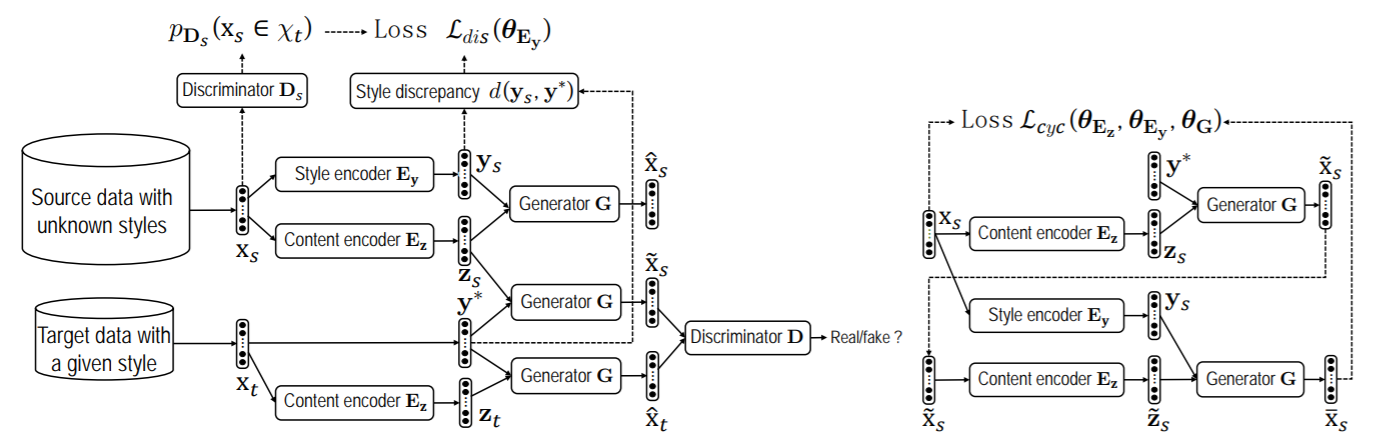
\includegraphics[scale=0.55]{model.PNG}
  \caption{Model Diagram}
  \label{fig:model}
\end{figure}

There are four components to the overall loss function including reconstruction loss, adversarial loss, style discrepancy loss and cycle consistency loss. These components each serve to help the model make useful latent representations and generate sentences with transferred style. These four losses are combined into a single objective with parameters to tune the contribution of each component.

The reconstruction loss encourages the model to reconstruct the input. This loss function measures how well the source sentence can be recreated from only its style and content representations. The purpose of this loss is to generate accurate representations of the style and content. 

The adversarial loss encourages the generated sentence to have the same style as the target domain. A discriminator is a classifier trained to distinguish between the real and fake sentences. The real sentence is that which was generated directly from $z_target$ and $y*$. The fake sentence is that which was generated from $z_source$ and $y*$. The generator (decoder) is trained to fool the discriminator by generating sentences that are indistinguishable from the target domain. 

A typical encoder-decoder structure would require a reconstruction loss and an adversarial loss to generate sentences that are similar to the target domain. However, the problem is under-constrained in two respects. First, the representations will not necessarily represent style and content unless they are explicitly told to do so. Second, the content may vary from the source sentence to the generated sentence. The following two losses address these two issues.

The style discrepancy loss tries to relate the style encoding of the target sentences with the style encoding of the source sentences. The style discrepancy is measured by taking the $l_2$ norm of $y_s$ and $y^*$. If this measure . In order to link this discrepancy to the actual style property of the data it need to be combined with a classifier that can actually detect differences in style. This classifier is a discriminator $D_s$ that is trained on a portion of the training data to predict the probability that a given sentence has the target language style. This probability is then multiplied by the style discrepancy to produce the final loss. This has the effect of making sure that the style representation corresponds to the actual style of the sentence and that the style is encouraged to be 

The cycle consistency loss encourages the generated sentence to preserve the content of the source sentence. 



%%%%%%%%%%%%%%%%%%%%%%%%%%%%%%%%%%%%%%%%%%%%%%%%%
\section{Datasets}
In order to directly compare our evaluation result with Zhao et al. (2018), we plan to use the same English datasets. 
\paragraph{Yelp}
This raw data is provided by Yelp in their Yelp Challenge Round 10, which contains restaurant reviews where 4/5 stars are considered positive, 1/2 stars negative, and 3 stars neutral. \newline
Preprocessed positive and negative data is released by Shen et al. (2017), which contains 250k negative sentences and 350k positive sentences.  \newline
For neutral reviews will be preprocessed using the same approach per Zhao et al. (2018). \newline
Finally 500k sentences will be sampled from the resulting dataset as the neutral data. We use the positive data as the target style domain. Based on the three classes of data, two source datasets are constructed with multiple styles:

\begin{itemize}
\item Positive+Negative (Pos+Neg): we add different numbers of positive data (50k, 100k, 150k) into
the negative data so that the source domain contains data with two sentiments.
\item Neutral+Negative (Neu+Neg): we combine neutral (50k, 100k, 150k) and negative data together as the source data.
\end{itemize}

\paragraph{Shakespeare}
We experiment on revising modern text in the Shakespearean style at the sentence-level as in (Mueller et al., 2017). Following their experimental setup, we collect 29,388 sentences authored by Shakespeare and 54,800 sentences from non-Shakespeare-authored works. The length of all the sentences ranges from 3 to 15. \newline

\paragraph{Split the Data}
Each of the datasets is divided into three non-overlapping parts which are respectively used for the style transfer model, the pre-trained discriminator (Ds), and the evaluation classifier (see \ref{eval}). Each part is further divided into training, testing, and validation sets. There is one exception that Ds for Shakespeare is trained on a subset of the data for training the style transfer model because the Shakespeare dataset is small. 

%%%%%%%%%%%%%%%%%%%%%%%%%%%%%%%%%%%%%%%%%%%%%%%%%
\section{Evaluation Metrics}
\label{eval}
Since the latent representation is decomposed into style variable and content variable (see \ref{representation}), it follows naturally that the two general evaluation metrics we'll be using are transfer strength and content preservation (Fu et al.(2017)).

\subsection{Transfer Strength}
Transfer strength evaluates whether the style is transferred and is implemented using a \texttt{LSTM-sigmoid} classifier which performs well on big data. The style is defined in \ref{style}. This classifier is based on keras examples\footnote{
https://github.com/fchollet/keras/blob/master/examples/imdb-lstm.py}. Transfer strength accuracy is defined as $\frac{Nright}{Ntotal}$, $Ntotal$ is the number of test data, and $Nright$ is the number of correct case which
is transferred to target style.

\begin{equation}
\label{style}
  l_{style} =
    \begin{cases}
      paper(positive) & \text{output <= 0.5}\\
      news(negative) & \text{output > 0.5}
    \end{cases}       
\end{equation}

\subsection{Content Preservation}
Another important aspect of style transfer is content preservation, where we evaluate the similarity between source text and target text. Content preservation rate is defined as cosine distance \ref{cosine} between source sentence embedding $v_s$ and target sentence embedding $v_t$. Sentence embedding consists of \texttt{max,min,mean} pooling of word embedding defined in \ref{embeddings}.
\label{cosine}
\begin{equation}
    score = \frac{v_{s}^T v_{t}}{\norm{v_s}\norm{v_t}}
\end{equation}

\label{embeddings}
\begin{equation}
\begin{aligned}
    v_{min}[i] & = min\{w_1[i], ... w_n[i]\} \\
    v_{mean}[i] & = mean\{w_1[i], ... w_n[i]\} \\
    v_{max}[i] & = max\{w_1[i], ... w_n[i]\} \\
    v & = [v_{min}, v_{mean}, v_{max}]
\end{aligned}
\end{equation}

\section*{References}

\medskip

\small

[2018] Zhao, Bi, Wei, Cai, Liu, Xiaojiang, Tu \ \& Shi \ Language Style Transfer from Sentences with Arbitrary Unknown Styles. {\it arXiv:1808.04071v1}

[2013] Yan, R.; Jiang, H.; Lapata, M.; Lin, S.-D.; Lv, X.;  \ \& Li, X. 2013. i, poet: Automatic chinese poetry composition through a generative summarization framework under constrained optimization. {\it IJCAI, 2197 $-$2203.}

[2016] Yan, R. 2016. i, poet: Automatic poetry composition through recurrent neural networks with iterative polishing schema. {\it IJCAI, 2238 $-$2244}.

[2016] Ghazvininejad, M.; Shi, X.; Choi, Y.; and Knight, K. 2016. Generating topical poetry. {\it EMNLP, 1183$-$1191}

[2017] Shen, Tianxiao; Lei, Tao; Barzilay, Tianxiao \ \$ Jaakkola, Tommi. Style Transfer from Non-Parallel Text by Cross-Alignment. {\it NIPS 2017. arXiv}

[2017] Fu, Zhenxin; Tan, Xiaoye; Peng, Nanyun; Zhao, Dongyan; Yan, Rui. Style Transfer in Text: Exploration and Evaluation {\it arXiv:1711.06861v2 }

\end{document}
